\documentclass[11pt]{article}
\usepackage[margin=0.85in]{geometry}
\usepackage{amsmath,amssymb,booktabs,longtable,graphicx,hyperref}
\hypersetup{colorlinks=true,linkcolor=blue,urlcolor=blue}
\setlength{\emergencystretch}{3em}
\title{E-Cigarette Supply: A Conference-Version Model}
\author{Erin Eidschun}
\date{Draft --- reconstructed and revised October 27, 2026}
\begin{document}
\maketitle
\begin{center}\textit{Motivating facts, model environment, and equilibrium definition.\\Static pricing, exogenous state, explicit passive fringe.}\end{center}
\paragraph{Revision record.} Reconstructed from the archived PDF; duplicate and overlapping text has been consolidated. Demand now uses the signed coefficient $\alpha<0$ multiplying $+p$. Fringe mean utility includes price and unobserved quality and is calibrated to observed shares for initial replication. The October 7 construction and concentration diagnostics below are historical records, not newly recomputed statistics. Original PDFs are retained in \texttt{source\_archive/pre\_reconstruction/}.

\section{Motivating facts}
The tracked e-cigarette market is small-$N$ and its leadership turns over. Figure~\ref{fig:composition} plots annual, mL-weighted brand composition from the Nielsen RMS panel: the top five brands each year, individually shaded, with the market leader starred and everyone else pooled into ``Other.''
\begin{figure}[htbp]\centering
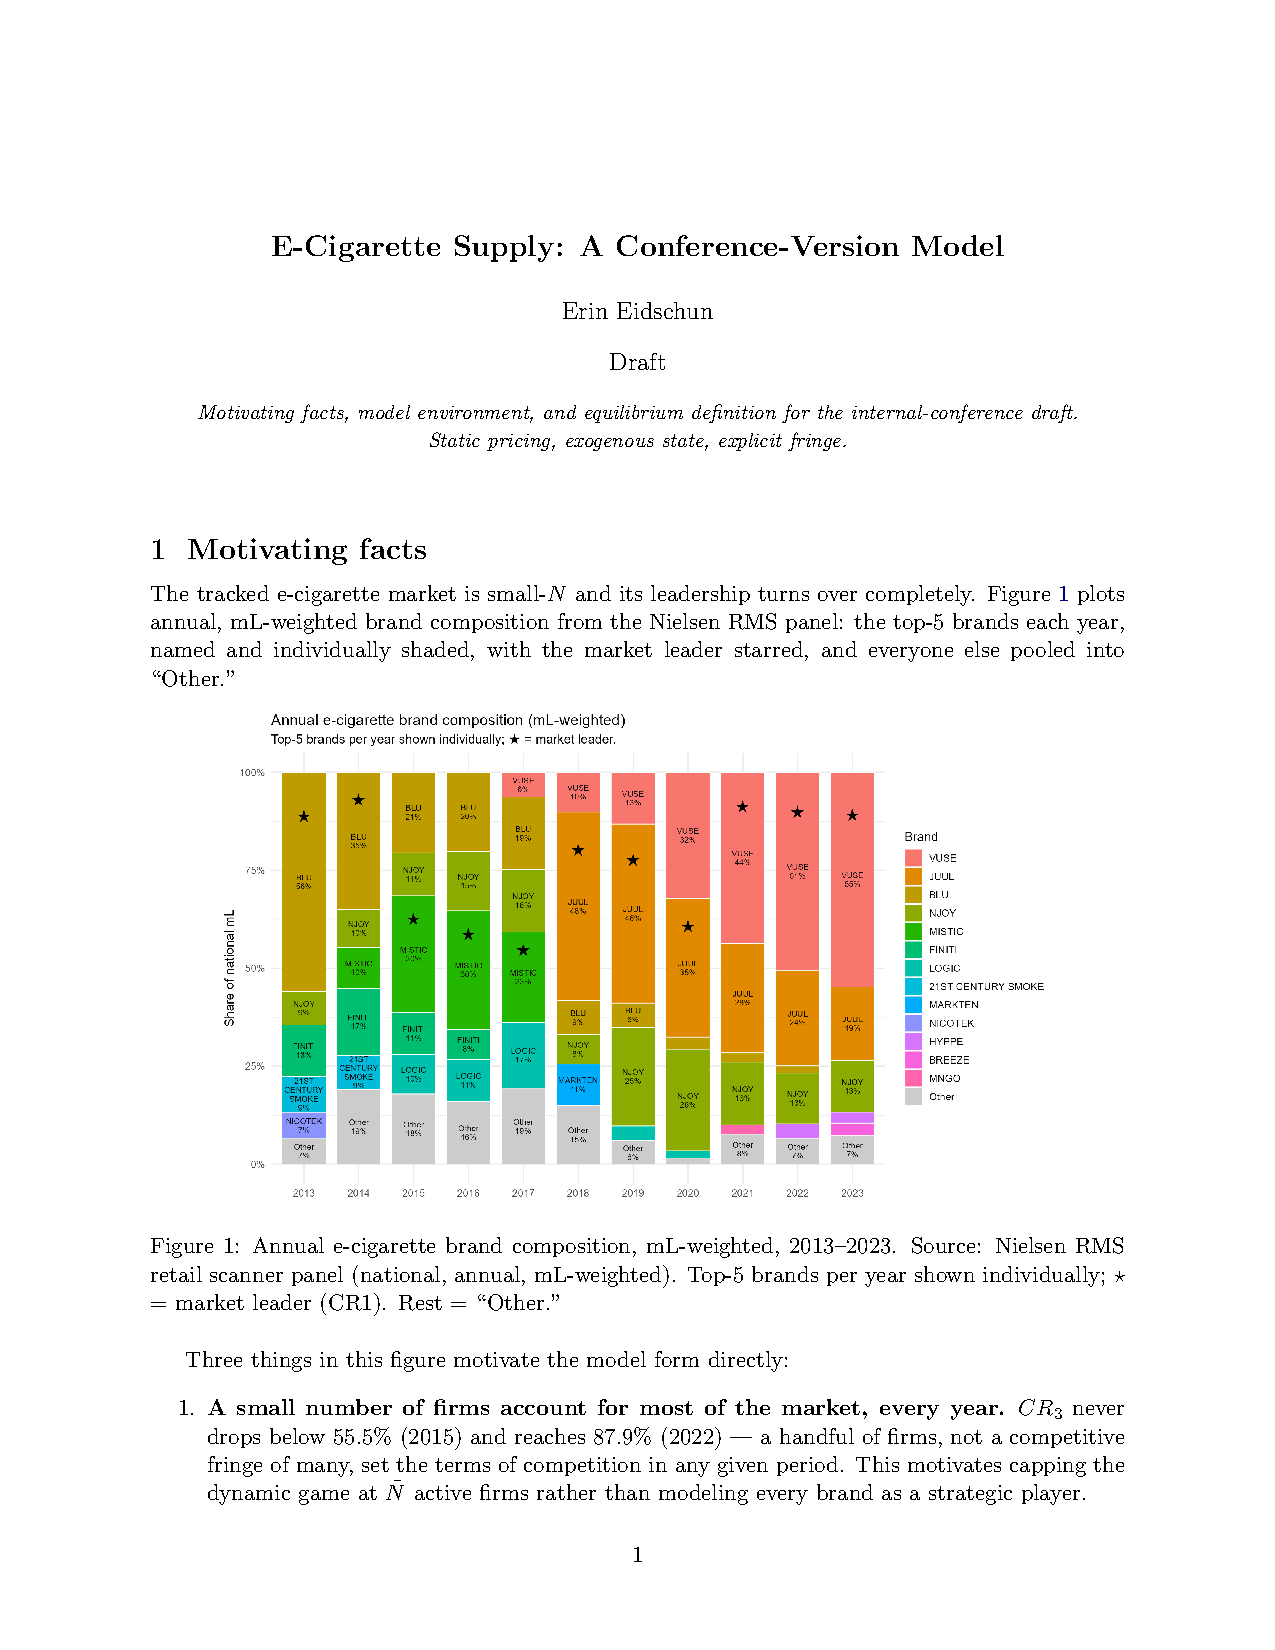
\includegraphics[page=1,trim=70 210 65 340,clip,width=0.92\linewidth]{source_archive/pre_reconstruction/ec_supply_conference_model.pdf}
\caption{Annual e-cigarette brand composition, mL-weighted, 2013--2023. Original figure retained from the archived model PDF. Source: Nielsen RMS national retail scanner panel. Top five brands per year; star denotes the market leader; rest pooled as Other.}\label{fig:composition}
\end{figure}
Three patterns motivate the model:
\begin{enumerate}
\item A small number of firms account for most sales. Historical CR3 ranges from 55.5\% (2015) to 87.9\% (2022), motivating a finite set of strategic incumbents rather than treating every brand as a strategic player.
\item Leadership changes: BLU (2013--2014), MISTIC (2015--2017), JUUL (2018--2020), and VUSE (2021--2023). Entry, exit, and eventually investment can be studied in a dynamic model rather than inferred from a single cross-section.
\item The residual group is persistent and varies over time. Distinguish sales below CR3 from the model's fringe, which is defined by the incumbent-share rule. The old text says the below-CR3 group is approximately 12--22\% in most years and 12.3\% in 2020, and cites a companion August 27 diagnostic reporting 15--22\% through 2014--2018. These claims do not match the transcribed CR3 table: the complement is 44.5\% in 2015 and 12.7\% in 2020. Different residual definitions or source vintages may be involved; those historical claims require reconciliation rather than being silently applied to the current fringe.
\end{enumerate}
\begin{table}[htbp]\centering\small
\begin{tabular}{llrlrr}\toprule
Year&Leader&Leader share&Runner-up&CR3&HHI\\\midrule
2013&BLU&56.0\%&FINITI&78.3\%&3519\\
2014&BLU&35.0\%&FINITI&61.8\%&1869\\
2015&MISTIC&24.0\%&BLU&55.5\%&1430\\
2016&MISTIC&25.9\%&BLU&61.3\%&1564\\
2017&MISTIC&20.8\%&BLU&56.0\%&1430\\
2018&JUUL&46.9\%&VUSE&67.7\%&2612\\
2019&JUUL&42.3\%&NJOY&77.0\%&2609\\
2020&JUUL&33.7\%&VUSE&87.3\%&2639\\
2021&VUSE&43.7\%&JUUL&87.7\%&2966\\
2022&VUSE&50.5\%&JUUL&87.9\%&3338\\
2023&VUSE&54.8\%&JUUL&86.8\%&3553\\\bottomrule
\end{tabular}
\caption{Historical national concentration diagnostics, mL-weighted; transcribed from the original PDF.}
\end{table}
HHI is U-shaped in the historical table: approximately 3,500 initially, 1,400--1,600 during 2015--2017, and higher again after 2018. This motivates studying turnover but does not by itself identify its cause. The original discussion linked the timing to salt-nicotine innovation and FDA actions; those are hypotheses rather than causal estimates from this table.

\section{Environment}
\paragraph{Players and timing.} Period $t$ is a month. A finite set $I_t$ of incumbents prices strategically, alongside one aggregate passive fringe $F$ and at most one potential entrant in the dynamic extension. Each period: states are realized; incumbents set prices conditional on the fringe utility; profits realize; incumbents choose continuation/exit and the potential entrant chooses entry; states evolve into $t+1$.
\paragraph{State.} Incumbent $i$ carries $\omega_{i,t}=(a_{i,t},\xi_{i,t})$: observed delivered nicotine concentration and an unobserved demand component. The conference draft proposes exogenous first-order laws
\[
a_{i,t+1}\sim F_a(\cdot\mid a_{i,t}),\qquad
\xi_{i,t+1}\sim F_\xi(\cdot\mid\xi_{i,t}).
\]
Independence between these processes and pooling across firms are proposed simplifications, not implications of the data. No transition estimation is required for an observed-month static solve. The initial solve conditions on current $a$, $\xi$, costs, roster, market size, and $\delta_{F,t}$. With the revised fringe, its quality alone is not a sufficient dynamic state: a future law for total fringe utility, or its components, remains to be specified.
\paragraph{Roster versus cap.} The historical draft proposes $\bar N=5$ strategic firms in the dynamic game. Empirical demand instead classifies brands with annual eligible volume share strictly above 7\% as incumbents, keeping that roster fixed through the year. The reported annual count ranges from three to six. Thus five cannot be called nonbinding in six-incumbent years. Static replication should retain its observed demand roster; the dynamic cap and treatment of six-firm observations remain unresolved.

\section{Demand}\label{sec:demand}
Incumbents and the fringe occupy one e-cigarette nest $g$, with an outside option normalized to mean utility zero. Use the same signed-alpha convention as current estimation:
\begin{equation}
\delta_{i,t}=c+\beta_a a_{i,t}+\xi_{i,t}+\alpha p_{i,t},\qquad \alpha<0,\quad 0\leq\sigma<1.
\end{equation}
Here $c$ is an intercept, distinct from marginal cost $mc_i$. The coefficient $\beta_a$ is estimated, not normalized to one: nicotine is measured on a physical scale. The original draft motivates a free quality coefficient with Ericson--Pakes and uses the Berry mean-utility interpretation. The residual $\xi_{i,t}$ is a brand-month demand component, not an individual consumer's taste disturbance.
Define
\begin{align}
D_{g,t}&=\sum_{j\in I_t\cup\{F\}}\exp\!\left(\frac{\delta_{j,t}}{1-\sigma}\right),&
s_{i\mid g,t}&=\frac{\exp(\delta_{i,t}/(1-\sigma))}{D_{g,t}},\\
IV_{g,t}&=(1-\sigma)\log D_{g,t},&s_{g,t}&=\frac{\exp(IV_{g,t})}{1+\exp(IV_{g,t})},\\
s_{i,t}&=s_{i\mid g,t}s_{g,t},&s_{0t}&=1-s_{g,t}.
\end{align}
The inverted demand equation is
\begin{equation}\label{eq:inversion}
\log(s_{i,t}/s_{0t})=c+\alpha p_{i,t}+\beta_a a_{i,t}+\sigma\log(s_{i,t}/s_{g,t})+\xi_{i,t}.
\end{equation}
Price and within-nest log share are instrumented jointly; current quality is treated as exogenous in the selected provisional model.
\paragraph{Historical retail construction.} The October 7 rebuild defines each UPC-month price as real revenue divided by corrected mL, filters to positive units/volume, known brands, and at least three reporting stores nationally, and takes an equal-UPC firm mean. Reviewed pack counts/capacities update volume, nicotine quantities, and shares; the separate NCP household input stays unchanged. For $\bar p=N^{-1}\sum_u p_u$, $Q=\sum_u q_u$, and $R=\sum_u p_uq_u$,
\[
\bar pQ-R=\sum_u(\bar p-p_u)q_u,
\]
which generally differs from zero. The separate liquid-volume-weighted price $R/Q$ recovers revenue exactly.
\paragraph{Current provisional specification.} Following the October 26 meeting and October 27 selection, use liquid-volume-weighted prices, no firm FE, nicotine only, and constant NCP purchasing intensity times annual adult population. The 528-row specification estimates $c=-6.893768$, $\alpha=-0.333588$, $\beta_a=0.110019$, $\sigma=0.869476$. The excluded instruments are current brand-specific sales-volume-weighted state tax and annual national incumbent count. This is a provisional choice, not a validated structural calibration; its tax--price association remains negative and its sigma interval extends above one. Historical diagnostics also compare device size, log UPC variety, population-weighted taxes, and national/geographic active-brand counts. SEs are clustered by month; there are no month FE.

\paragraph{Historical instrument definitions and exclusions.} Before the current sales-weighted-tax comparison, the tax instrument was
\[
\mathrm{Tax}^{\mathrm{pop}}_{it}=\sum_{s\in S_{it}}
\frac{\mathrm{Pop}_{s,t}}{\sum_{s'\in S_{it}}\mathrm{Pop}_{s',t}}\,\tau_{s,t},
\]
where $S_{it}$ is the firm's operating-state set. The national active-brand count counts all eligible active brands; the geographic version counts distinct brands operating in the union of the firm's states. Both include the focal brand and fringe brands. Historical specifications compare with/without firm FE, no month FE, and month clustering; these counts differ from the annual incumbent count in the selected specification. Diagnostic capacity is the equal-UPC mean mL per cartridge/disposable, while log variety counts all eligible UPCs. Matched control comparisons exclude and report firm-months with incomplete device-size coverage. Relevance and exclusion are separate questions; no sigma admissibility constraint was imposed during demand estimation.

\section{Static pricing subgame}
Each incumbent takes rivals' prices and fringe utility as given and maximizes
\begin{equation}
\pi_i(p;\Omega_t)=(p_i-mc_i)M_ts_i(p;\Omega_t)-FC_i.
\end{equation}
For an interior optimum, $s_i+(p_i-mc_i)\partial s_i/\partial p_i=0$. Let
\[
A_i(p)=\frac{1}{1-\sigma}-\frac{\sigma}{1-\sigma}s_{i\mid g}(p)-s_i(p).
\]
Then the simultaneous markup equations are
\begin{equation}
p_i=mc_i-\frac{1}{\alpha A_i(p)}=mc_i+\frac{1}{(-\alpha)A_i(p)}.
\end{equation}
The market-size factor cancels from the FOC conditional on the demand utilities; market-size assumptions still affect estimated demand and recovered utilities. Fixed operating costs affect profit levels, not interior optimal prices. One strategic product per brand and effective constant marginal cost per mL are maintained here; each brand is modeled as a vertically integrated pricing firm choosing its representative retail price and receiving the corresponding retail revenue. Recovered marginal costs are effective integrated-channel costs, and profits are integrated-channel profits rather than separately identified manufacturer profits. No separate wholesale-price or retailer-margin game is modeled.

The initial exercise recovers $\xi_{i,t}$ and marginal costs at observed prices and manually solves for prices holding those inputs fixed. This is an implementation replication, not independent validation. Use a transparent damped markup fixed point with share, price-step, and FOC checks, and unilateral profit-deviation checks before reporting a Nash equilibrium. No packaged black-box equilibrium solver is to be used. The appendix gives the equations and algorithm. Pricing is static: continuation values do not enter current FOCs under the maintained exogenous-state specification.

\section{Dynamic entry and exit}
This section records the proposed extension; no dynamic assumptions have been newly selected for the initial static exercise. Let $\pi_i^*(\Omega_t)$ be static equilibrium profit. With post-profit exit decisions,
\begin{equation}
V_i(\omega_{i,t},\omega_{-i,t})=\pi_i^*(\Omega_t)+
\max\left\{\phi_i,\ \beta\,\mathbb E[V_i(\Omega_{t+1})\mid\Omega_t,i\text{ continues}]\right\}.
\end{equation}
The incumbent exits if scrap value exceeds continuation value:
\[
\lambda_i^{\mathrm{exit}}=\mathbf 1\{\phi_i>\beta\mathbb E[V_i(\Omega_{t+1})\mid\Omega_t,i\text{ continues}]\}.
\]
A potential entrant draws initial state $\omega_{e,0}\sim G_e$ and enters for next-period operation if
\[
\lambda^{\mathrm{entry}}=\mathbf 1\{\beta\mathbb E[V_e(\omega_{e,0},\omega_{-e,t+1})\mid\Omega_t]-x_e\geq0\}.
\]
The notation $\lambda$ avoids conflict with nesting $\sigma$ and other shocks used in related papers. Rivals' exit and possible entry affect the continuation expectation through the transition kernel and equilibrium policies; their effects are not ignored simply because pricing is static.

\paragraph{Unresolved information structure.} The original draft alternates between fixed/known $\phi_i,x_e$ and private random draws. Under the former, policies are deterministic conditional on state. Under the latter, policies conditional only on public state are probabilities obtained by integrating over specified shock distributions. The distributions, timing, cap treatment, and resulting expected-max Bellman equation must be specified before dynamic implementation. The appendix's worked deterministic-policy example is conditional on that information structure, not a commitment for estimation.
\paragraph{Exit sample.} The historical notes identify MarkTen's 2018 discontinuation and MISTIC's approximately 2020 wind-down as possible parent-company/ownership exits, to be distinguished from endogenous demand-state exits. The original draft explicitly carves these out as exogenous ownership shocks and proposes using the remaining top-five exits to identify scrap values. This records the historical sample decision; the classifications and their identifying implications require confirmation against current data before estimation.

\section{The fringe}
The original $a_{F,t}$ is an equal-UPC average of delivered nicotine across active fringe UPCs, constructed from data rather than inferred from the demand regression. The passive fringe is an aggregate alternative with
\begin{equation}
\delta_{F,t}=c+\beta_a a_{F,t}+\alpha p_{F,t}+\xi_{F,t}.
\end{equation}
For initial replication, infer its total utility directly from observed shares:
\begin{equation}
\delta_{F,t}^{\mathrm{obs}}=\log(s_{F,t}/s_{0t})-\sigma\log(s_{F,t}/s_{g,t}),\qquad
\xi_{F,t}=\delta_{F,t}^{\mathrm{obs}}-c-\beta_a a_{F,t}-\alpha p_{F,t}.
\end{equation}
Its price and quality aggregates must be consistently defined to interpret this decomposition; total calibrated utility suffices for the static solve. Hold $\delta_{F,t}$ fixed while incumbent prices change. Its share changes endogenously through $D_{g,t}$ and $s_{g,t}$, but it has no strategic pricing FOC or Bellman equation. Utility can vary across months. This replaces the historical restriction $\delta_F=\beta_a a_F$; measured quality alone need not fit observed fringe shares. A future dynamic law for fringe utility remains an open choice.

\section{What this version leaves for later}
\begin{itemize}
\item \textbf{Investment.} Quality is exogenous here. The full draft proposes a binary investment choice, firm-time investment costs $\kappa_{\mathrm{inv},i,t}$, and stochastic success. It proposes Experience-Based Equilibrium for the larger state space, following the discussion with Ariel Pakes. FDA enforcement dates and a JUUL-specific increment could enter investment costs, allowing rivals' continuation values to respond, rather than imposing only a direct quality cap. These are proposed extensions.
\item \textbf{Quality's cost channel.} The old discussion reports no price-identified learning-cost signature for JUUL/VUSE/NJOY, only for the earlier cigalike cohort. Price alone does not separate marginal costs from markups. No nicotine-driven cost-reduction law is imposed here; marginal costs remain required inputs or recovered objects.
\item \textbf{Incumbent threshold and dynamic entry.} Does crossing the annual 7\% share threshold count as economic entry/exit, or only a change in the demand roster? The old diagnostic reports unbroken incumbent spells at 7\%, but NJOY falls below a 10\% threshold in 2018 (reported 7.6\%) and returns subsequently. Reclassification and actual sales entry/exit must be distinguished. Six-incumbent years also require resolving the proposed five-firm cap.
\item \textbf{A strategic fringe.} A future model could replace the passive aggregate with a strategic or free-entry sector. That is not implemented by calibrating $\xi_F$.
\item \textbf{Legacy-brand bias in fringe quality.} Historical diagnostics report post-exit MarkTen UPCs raising $a_F$ by approximately 12--20\% through 2019 and NICOTEK lowering it by approximately 10--11\%, with other tracked firms' post-exit residual effects reported negligible. A proposed correction excludes post-exit UPCs when deviations exceed about 10\%, preserving pre-incumbency histories of rising brands such as JUUL/VUSE. The original draft says this correction was validated but not implemented. Its status and the 2021 panel-onboarding adjustment should be checked against current builders before use; no correction is applied by this reconstruction.
\item \textbf{Ownership, nicotine costs, and vertical structure.} The functional meaning of nicotine-related costs and ownership-driven turnover remain open. Effective retail-cost recovery does not by itself identify manufacturer technology or tax incidence.
\end{itemize}

\section{Framework and references}
The original draft cites Ericson \& Pakes (1995) for the dynamic framework; Pakes \& McGuire (1994, 2001) for computation and recurrent-state methods; Fershtman \& Pakes (2012) for Experience-Based Equilibrium; Spence (1981) for learning by doing; and Benkard (2000, 2004) for aircraft-manufacturing applications. The original text also cites Ericson--Pakes (1994) in discussing the static profit/quality coefficient. Berry (1994), BLP, and Train motivate demand inversion and nested-logit shares. These attributions are retained as draft references, not newly verified bibliographic claims; resolve the Ericson--Pakes year discrepancy and full citations before submission.
\end{document}
